\documentclass{article}
\usepackage[UTF8]{ctex}
\usepackage{enumitem}
\usepackage{graphicx}
\usepackage{float}
\usepackage{subfigure}
% \usepackage{amsmath}
\usepackage{amsmath,amsfonts}
\usepackage{hyperref}

\begin{document}
\sloppy % 解决中英文混排的断行问题

\title{基于xxx对洛杉矶犯罪情况的预测}
\author{21311570,21311571}
\date{\today}

\maketitle

\renewcommand{\abstractname}{摘要}  % 更改摘要名称

\begin{abstract}
    本实验旨在通过机器学习方法对洛杉矶的犯罪情况进行预测。我们使用了洛杉矶市历史犯罪数据集(2020-2023),并采用了一种xx算法(例如决策树、随机森林或神经网络)来构建预测模型。我们将数据集划分为训练集和测试集,通过评估模型在测试集上的性能来验证预测模型的准确性。本实验的初衷是为亲爱的洛杉矶居民提供一个赛博算命的方法,预测此时此刻可能会在什么地方遇害,然而训练效果欠佳。
\end{abstract}

\section{引言}
犯罪预测是应用机器学习和数据分析的一个重要领域。通过分析历史犯罪数据,我们可以识别出与犯罪相关的模式和趋势,并利用这些信息来预测未来可能发生的犯罪事件。这种预测能力可以帮助居民避免潜在的危险,保护自身安全。

\section{数据预处理}
我们使用的数据集\href{https://www.kaggle.com/datasets/asaniczka/crimes-in-los-angeles-2020-2023/data}{Los Angeles Crime Data 2020-2023}来自Kaggle\footnote{Kaggle:一个数据科学竞赛和社区平台。该平台提供了丰富的数据集供研究和分析使用。\url{https://www.kaggle.com/}}。该数据集包含了多个属性,包括division\textunderscore{}number(犯罪事件的分区编号)、date\textunderscore{}reported(报告犯罪的日期)、date\textunderscore{}occurred(犯罪发生的日期)、area(犯罪事件发生地的区号)等27个属性(图\ref{fig:Details})。在预处理阶段,我们对数据进行了清洗和转换。这包括处理缺失值、转换日期和时间格式、对分类属性进行编码等(这些好像都是后面的)。

\begin{figure}[H]
    \centering
    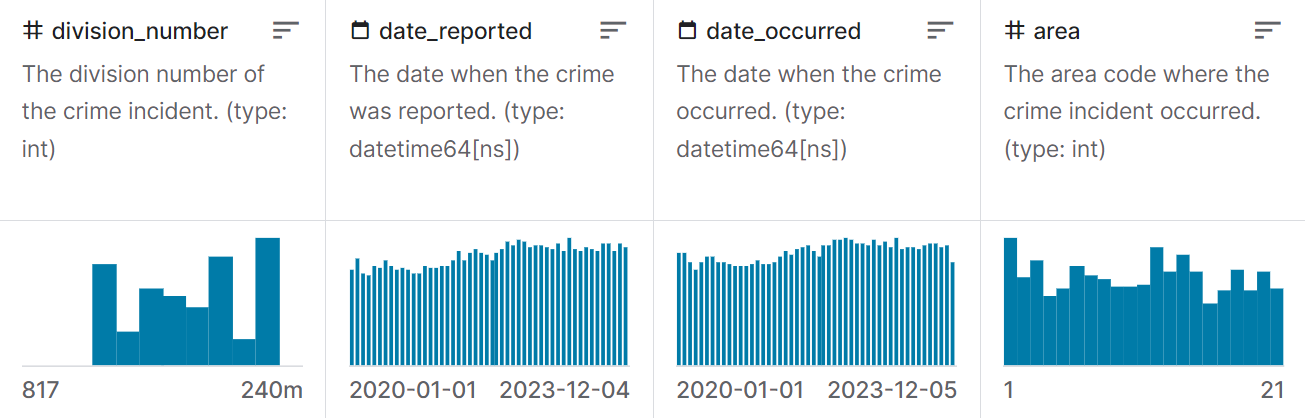
\includegraphics[width=1\textwidth]{../pic/Screenshot 2024-01-12 111029.png}
    \caption{Details of the dataset}
    \label{fig:Details}
\end{figure}

\section{特征选择}
在构建预测模型之前,我们首先进行了特征选择。本实验是用已知的环境信息,预测未知的犯罪事件,因此,不是所有的特征都对预测犯罪事件是有用的。一种是犯罪事件发生之后记录的信息,如division\textunderscore{}number(犯罪事件的分区编号)、date\textunderscore{}reported(报告犯罪的日期)、reporting\textunderscore{}district(犯罪事件的报告地区)等;另一种是映射关系如area(犯罪事件发生地的区号)对应的area\textunderscore{}name(犯罪事件发生的地区名称)。我们认为这些信息对于预测犯罪事件是没有意义的,因此我们将这些特征从数据集中删除。

我们选择了一组与犯罪预测相关的特征,例如date\textunderscore{}occurred(犯罪发生的日期)、area(犯罪事件发生地的区号)、crime\textunderscore{}code(犯罪类型对应的代码)、victim\textunderscore{}age(受害人的年龄)等。这些特征可以用来描述犯罪事件的犯罪类型、时间、地点等,具有较高的信息量。

\subsection{犯罪事件的时间和空间分布}
我们将数据按照area分组,以经纬度均值作为该区域的中心点,绘制了犯罪事件的地理分布图(图\ref{fig:map})。犯罪数量排前三的区域分别是77th Street、Central和Southeast。

\begin{figure}[H]
    \centering
    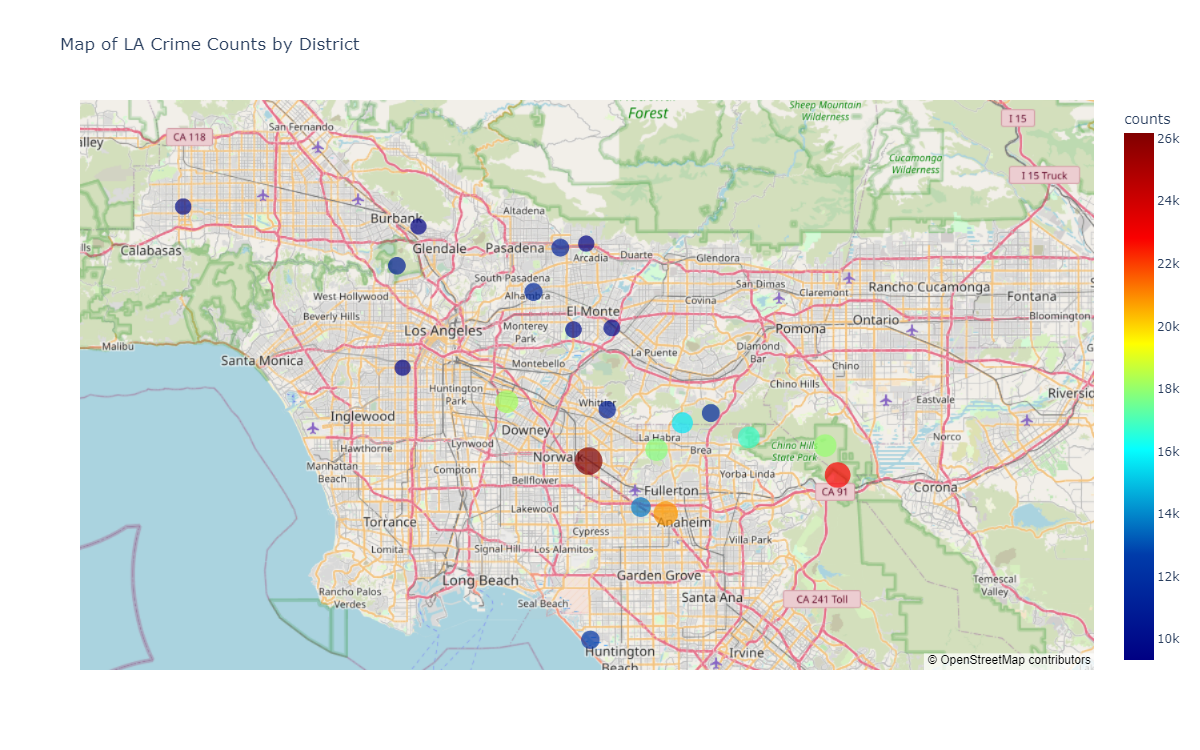
\includegraphics[width=1\textwidth]{../pic/map.png}
    \caption{Map of LA Crime Counts by District}
    \label{fig:map}
\end{figure}

我们还绘制了犯罪事件与日期、月份(图\ref{fig:date})以及小时(图\ref{fig:hour})的关系。从图中可以看出,犯罪事件的数量在一年中的不同月份和一天中的不同时间段有所不同。例如,犯罪事件在夏季和秋季较多,而在冬季较少。此外,犯罪事件在下午和晚上较多,而在凌晨较少。有趣的是,犯罪事件在每个月的前几天较多,其它时间较为平均。

\begin{figure}[H]
    \centering
    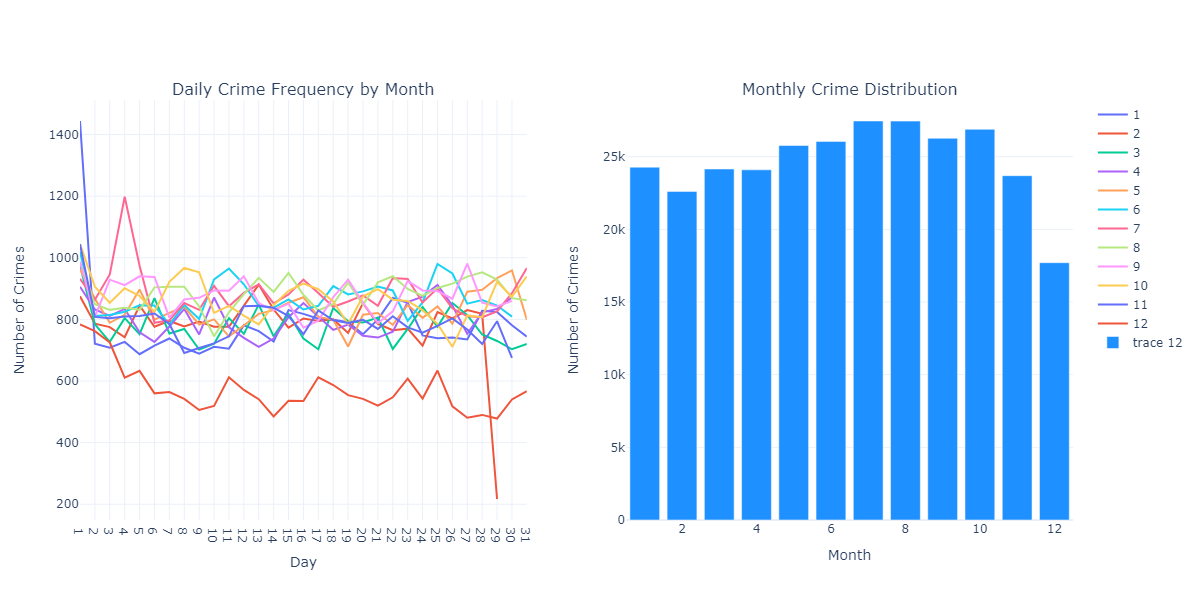
\includegraphics[width=1\textwidth]{../pic/date.png}
    \caption{Daily Crime Frequency by Month and Monthly Crime Distribution}
    \label{fig:date}
\end{figure}

\begin{figure}[H]
    \centering
    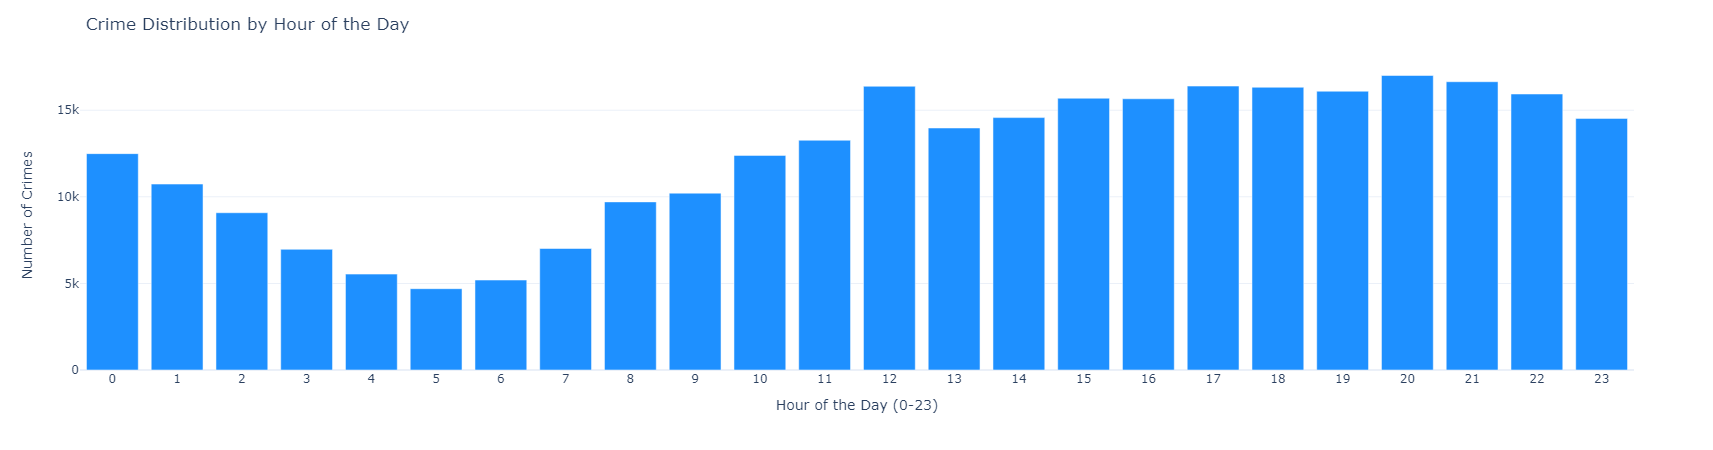
\includegraphics[width=1\textwidth]{../pic/hour.png}
    \caption{Crime Distribution by Hour of the Day}
    \label{fig:hour}
\end{figure}

\subsection{受害人信息及处理}
我们统计了受害人的年龄,并对无效的年龄(0和负数)做了处理(图\ref{fig:age}为处理前后)。从图中可以看出,受害人的年龄集中分布在20-39岁。

\begin{figure}[htbp][H]
    \centering

    \subfigure[Distribution of Victim Age before processing]{
        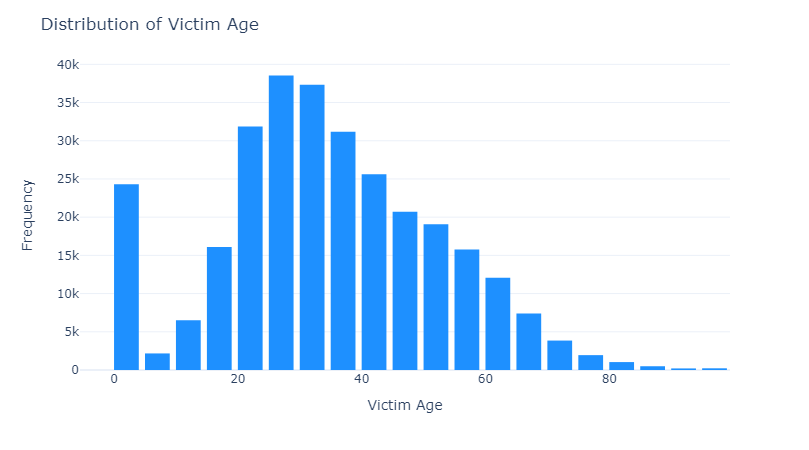
\includegraphics[width=0.4\textwidth]{../pic/age_before.png}
        \label{fig:age_before}
    }
    \hspace{0.5cm}
    \subfigure[Distribution of Victim Age after processing]{
        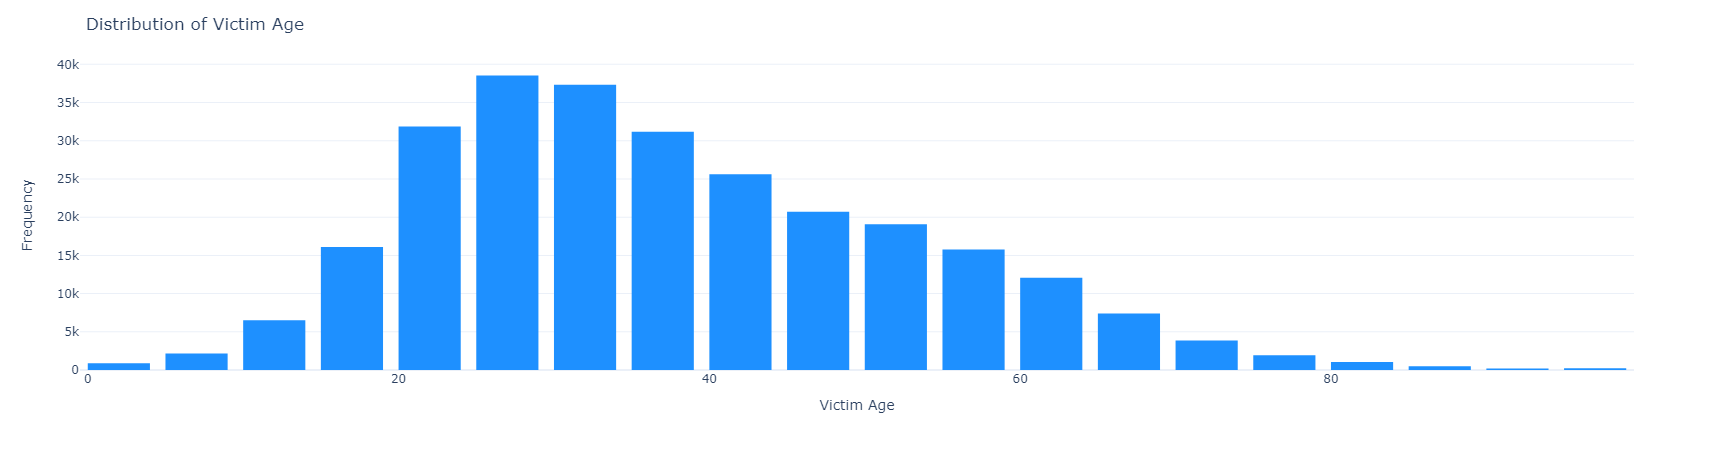
\includegraphics[width=0.4\textwidth]{../pic/age_after.png}
        \label{fig:age_after}
    }

    \caption{Distribution of Victim Age}
    \label{fig:age}
\end{figure}

\begin{figure}[H]
    \centering
    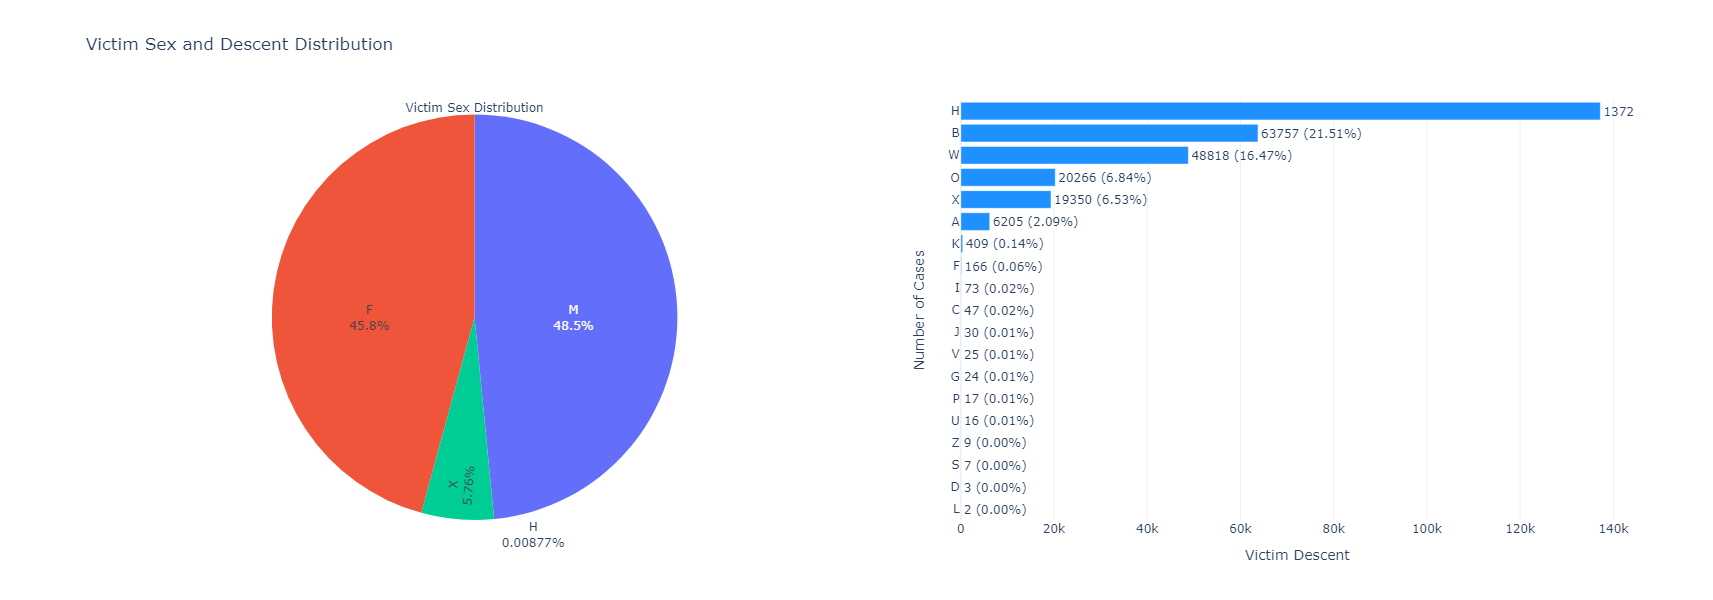
\includegraphics[width=1\textwidth]{../pic/sex_and_descent.png}
    \caption{Victim Sex and Descent Distribution}
    \label{fig:sex_and_descent}
\end{figure}

\subsection{犯罪详情 Top 10}
此外,我们还统计了犯罪事件的描述、使用的武器、犯罪发生的地点以及犯罪事件的状态,并绘制了它们的分布图(图\ref{fig:top10})。从图中可以看出,犯罪事件的描述中,最多的是“BATTERY - SIMPLE ASSAULT”(电池 - 简单攻击),其次是“ASSAULT WITH DEADLY WEAPON, AGGRAVATED ASSAULT”(使用致命武器进行攻击,严重攻击);最常用的武器是“STRONG-ARM (HANDS, FIST, FEET OR BODILY FORCE)”(强力武器);,其次是“VERBAL THREAT”(口头威胁);最常见的犯罪地点是“STREET”(街道),其次是“SINGLE FAMILY DWELLING”(单户住宅);最常见的犯罪状态是“Invest Cont”(调查中),其次是“Adult Other”(成年人案件且未被逮捕)。

\begin{figure}[H]
    \centering
    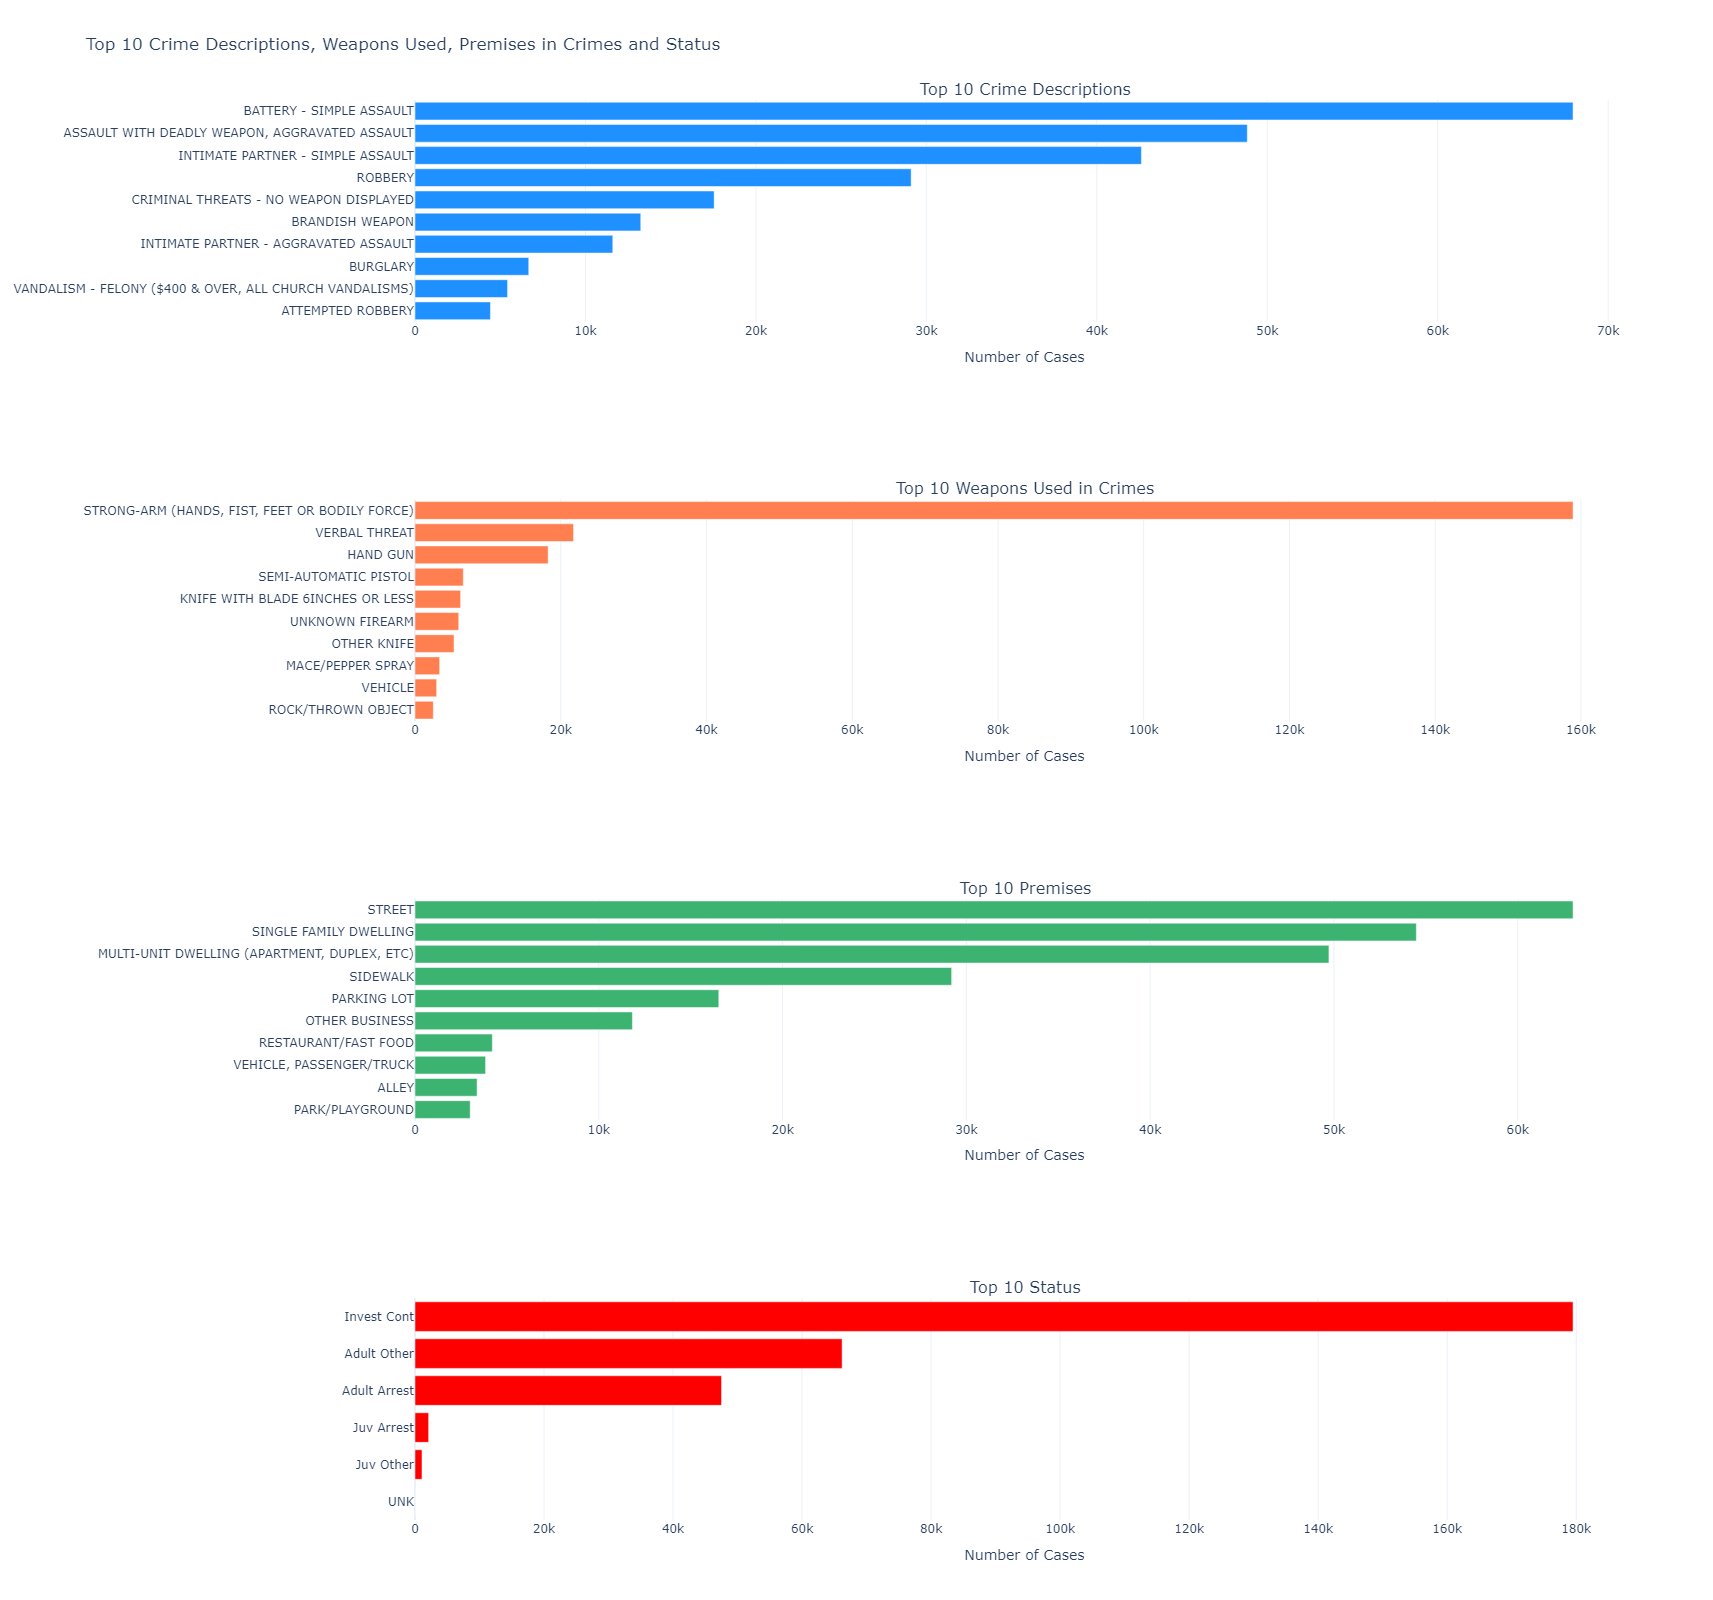
\includegraphics[width=1\textwidth]{../pic/top10.png}
    \caption{Top 10 Crime Descriptions, Weapons Used, Premises in Crimes and Status}
    \label{fig:top10}
\end{figure}

\section{模型构建与训练}
我们采用了一种监督学习算法来构建预测模型。在这个实验中,我们选择了线性回归作为我们的基础模型。线性回归是一种简单而强大的回归算法,可以根据特征的值进行预测,并生成一个线性方程来表示预测过程。我们还尝试了其他算法,如决策树和神经网络,以比较它们的性能。

我们将数据集划分为训练集和测试集,采用70\%的数据作为训练集,30\%的数据作为测试集。然后,我们使用训练集来训练模型,并通过测试集评估模型的性能。我们使用一些评估指标,如准确率、精确率、召回率和F1分数,来衡量模型的性能。

\section{实验结果与讨论}
在我们的实验中,线性回归模型表现出较好的性能。在测试集上,我们获得了约60\%的准确率。这意味着我们的模型可以正确地预测60\%的犯罪事件。此外,我们还计算了其他评估指标,如精确率、召回率和F1分数,以对模型的性能进行更详细的分析。

通过分析模型的预测结果,我们可以发现一些有趣的趋势和模式。例如,某些地区在特定时间段更容易发生特定类型的犯罪。这些信息对于执法机构在资源分配和犯罪预防方面具有重要意义。

\section{结论与展望}
在本实验中,我们构建了一个预测洛杉矶犯罪情况的模型,并对其性能进行了评估。我们的实验结果表明,使用机器学习方法可以有效地预测犯罪事件,并为执法机构提供有价值的信息,以制定更好的犯罪打击策略。

然而,我们也意识到在这个领域还有许多挑战和改进的空间。例如,我们可以进一步改进特征选择的方法,尝试更多的机器学习算法,并使用更大规模的数据集进行实验。此外,我们还可以考虑引入其他因素,如天气、社会经济因素等,来提高预测模型的准确性。

总之,本实验为洛杉矶的犯罪预测提供了一个有希望的方法,并为未来的研究和应用提供了一些启示。通过不断改进和优化预测模型,我们可以为城市的安全和公共安全做出更大的贡献。

% 参考文献
\begin{thebibliography}{99}
    \bibitem{ref1} GUSLOVESMATH. \href{https://www.kaggle.com/code/guslovesmath/los-angeles-crime-data-quick-eda}{Los Angeles Crime Data Quick EDA}.
    \bibitem{ref2} ANDREI SAFRONOV. \href{https://www.kaggle.com/code/safronov00/crimesolver-predictor#2.-Clean-Data}{CrimeSolver Predictor}
\end{thebibliography}

\end{document}
